\documentclass[
  a4paper,
  oneside,
  BCOR = 10mm,
  DIV = 12,
  12pt,
  headings = normal,
]{scrartcl}

%%% Length calculations
\usepackage{calc}
%%%

%%% Support for color
\usepackage{xcolor}
\definecolor{lightblue}{HTML}{03A9F4}
\definecolor{red}{HTML}{F44336}
%%%

%%% Including graphics
\usepackage{graphicx}
%%%

%%% Font selection
\usepackage{fontspec}

\setromanfont{STIX Two Text}[
  SmallCapsFeatures = {LetterSpace = 8},
]

\setsansfont{IBM Plex Sans}[
  Scale = MatchUppercase,
]

\setmonofont{IBM Plex Mono}[
  Scale = MatchUppercase,
]
%%%

%%% Math typesetting
\usepackage{amsmath}
\usepackage{mathtools}

\usepackage{unicode-math}
\setmathfont{STIX Two Math}

\usepackage{IEEEtrantools}
%%%

%%% List settings
\usepackage{enumitem}
\setlist[enumerate]{
  label*      = {\arabic*.},
  left        = \parindent,
  topsep      = 0\baselineskip,
  parsep      = 0\baselineskip,
  noitemsep, % override itemsep
}
% List settings for levels 2–4
\setlist[enumerate, 2, 3, 4]{
  label*      = {\arabic*.},
  left        = 0em,
  topsep      = 0\baselineskip,
  parsep      = 0\baselineskip,
  noitemsep, % override itemsep
}

\setlist[itemize]{
  label*      = {—},
  left        = \parindent,
  topsep      = 0\baselineskip,
  parsep      = 0\baselineskip,
  itemsep     = 1\baselineskip,
  noitemsep, % override itemsep
}

\setlist[description]{
  font        = {\rmfamily\upshape\bfseries},
  topsep      = 1\baselineskip,
  parsep      = 0\baselineskip,
  itemsep     = 0\baselineskip,
}

%%%

%%% Structural elements typesetting
\setkomafont{pagenumber}{\rmfamily\upshape}
\setkomafont{disposition}{\rmfamily\bfseries}

% Sectioning
\RedeclareSectionCommand[
  beforeskip = -1\baselineskip,
  afterskip  = 1\baselineskip,
  font       = {\normalsize\bfseries\scshape},
]{section}

\RedeclareSectionCommand[
  beforeskip = -1\baselineskip,
  afterskip  = 1\baselineskip,
  font       = {\normalsize\bfseries\itshape},
]{subsection}

\RedeclareSectionCommand[
  beforeskip = -1\baselineskip,
  afterskip  = 1\baselineskip,
  font       = {\normalsize\bfseries},
]{subsubsection}

\RedeclareSectionCommand[
  beforeskip = -1\baselineskip,
  afterskip  = -0.5em,
  font       = {\normalsize\mdseries\scshape\addfontfeatures{Letters = {UppercaseSmallCaps}}},
]{paragraph}
%%%

%%% Typographic enhancements
\usepackage{microtype}
%%%

%%% Language-specific settings
\usepackage{polyglossia}
\setmainlanguage{ukrainian}
\setotherlanguages{english}
%%%

%%% Captions
\usepackage{caption}
\usepackage{subcaption}

%\DeclareCaptionLabelFormat{closing}{#2)}
%\captionsetup[subtable]{labelformat = closing}

%\captionsetup[subfigure]{labelformat = closing}

\captionsetup[table]{
  aboveskip = 0\baselineskip,
  belowskip = 0\baselineskip,
}

\captionsetup[figure]{
  aboveskip = 1\baselineskip,
  belowskip = 0\baselineskip,
}

\captionsetup[subfigure]{
  labelformat = simple,
  labelformat = brace,
  justification = RaggedRight,
  singlelinecheck = false,
}
%%%

%%% Hyphenated ragged typesetting
\usepackage{ragged2e}
%%%

%%% Table typesetting
\usepackage{booktabs}
\usepackage{longtable}

\usepackage{multirow}

\usepackage{array}
\newcolumntype{v}[1]{>{\RaggedRight\arraybackslash\hspace{0pt}}p{#1}}
\newcolumntype{b}[1]{>{\Centering\arraybackslash\hspace{0pt}}p{#1}}
\newcolumntype{n}[1]{>{\RaggedLeft\arraybackslash\hspace{0pt}}p{#1}}
%%%

%%% Drawing
\usepackage{tikz}
\usepackage{tikzscale}
\usetikzlibrary{datavisualization}
\usetikzlibrary{datavisualization.formats.functions}
\usetikzlibrary{positioning}
\usetikzlibrary{patterns}
\usetikzlibrary{intersections}
\usetikzlibrary{arrows.meta} % Stealth arrow tips
\usetikzlibrary{graphs}
\usetikzlibrary{graphdrawing}
\usegdlibrary{layered}
\usetikzlibrary{quotes}

%%%

%%% SI units typesetting
\usepackage{siunitx}
\sisetup{
  output-decimal-marker = {,},
  exponent-product      = {\cdot},
  inter-unit-product    = \ensuremath{{} \cdot {}},
  per-mode              = symbol,
}
%%%

% Code Highlighting
\usepackage{minted}
\setmintedinline{
  style = bw,
  breaklines,
}

\newminted[bashterm]{text}{%
  autogobble,%
  breaklines,%
  style=bw,%
}

\newminted[codegeneric]{text}{%
  autogobble,%
  style=bw,%
  breaklines,%
  fontsize=\small,%
}

\newmintinline{bash}{%
}

\newmintinline[minttext]{text}{%
  breaklines,%
  breakanywhere,%
}

%%% Framing code listings
\usepackage{tcolorbox}
\tcbuselibrary{breakable}
\tcbuselibrary{minted}
\tcbuselibrary{skins}

% Text file listing
\newtcblisting[
  auto counter,
  list inside,
  number within = section,
]{listingplaintext}[3][]{%
  minted language = text,
  minted style    = bw,
  minted options  = {
    autogobble,
    linenos,
    tabsize = 4,
    breaklines,
    breakanywhere,
    fontsize = \footnotesize,
  },
  empty,
  sharp corners,
  coltitle = black,
  borderline horizontal = {1pt}{0pt}{black},
  titlerule = {0.5pt},
  titlerule style = {
    black,
  },
  toptitle = 0.3em,
  bottomtitle = 0.3em,
  before skip      = \intextsep,
  after  skip      = \intextsep,
  title            = {Лістинг \thetcbcounter: #2},
  list entry       = {\protect\numberline{\thetcbcounter}#2},
  left = 0em,
  right = 0em,
  %
  listing only,
  breakable,
  %
  label = {#3},%
}

\newtcbinputlisting[
  use counter from = listingplaintext,
  list inside,
  number within = section
]{\inputplaintext}[4][]{%
  minted language = text,
  minted style    = bw,
  minted options  = {
    autogobble,
    linenos,
    tabsize = 4,
    breaklines,
    breakanywhere,
    fontsize = \footnotesize,
  },
  empty,
  sharp corners,
  coltitle = black,
  borderline horizontal = {1pt}{0pt}{black},
  titlerule = {0.5pt},
  titlerule style = {
    black,
  },
  toptitle = 0.3em,
  bottomtitle = 0.3em,
  before skip      = \intextsep,
  after  skip      = \intextsep,
  title            = {Лістинг \thetcbcounter: #3},
  list entry       = {\protect\numberline{\thetcbcounter}#3},
  left = 0em,
  right = 0em,
  %
  listing file={#2},
  listing only,
  breakable,
  %
  label = {#4}
}

\newtcblisting[
  use counter from = listingplaintext,
  list inside,
  number within = section,
]{listingpython}[3][]{%
  minted language = python,
  minted style    = bw,
  minted options  = {
    autogobble,
    linenos,
    tabsize = 4,
    breaklines,
    breakanywhere,
    fontsize = \footnotesize,
  },
  empty,
  sharp corners,
  coltitle = black,
  borderline horizontal = {1pt}{0pt}{black},
  titlerule = {0.5pt},
  titlerule style = {
    black,
  },
  toptitle = 0.3em,
  bottomtitle = 0.3em,
  before skip      = \intextsep,
  after  skip      = \intextsep,
  title            = {Лістинг \thetcbcounter: #2},
  list entry       = {\protect\numberline{\thetcbcounter}#2},
  left = 0em,
  right = 0em,
  %
  listing only,
  breakable,
  %
  label = {#3},
  %
  #1%
}

\newtcbinputlisting[
  use counter from = listingplaintext,
  list inside,
  number within = section
]{\inputpython}[4][]{%
  minted language = python,
  minted style    = bw,
  minted options  = {
    autogobble,
    linenos,
    tabsize = 4,
    breaklines,
    breakanywhere,
    fontsize = \footnotesize,
  },
  empty,
  sharp corners,
  coltitle = black,
  borderline horizontal = {1pt}{0pt}{black},
  titlerule = {0.5pt},
  titlerule style = {
    black,
  },
  toptitle = 0.3em,
  bottomtitle = 0.3em,
  before skip      = \intextsep,
  after  skip      = \intextsep,
  title            = {Лістинг \thetcbcounter: #3},
  list entry       = {\protect\numberline{\thetcbcounter}#3},
  left = 0em,
  right = 0em,
  %
  listing file={#2},
  listing only,
  breakable,
  %
  label = {#4}
}

% Linux command-line listing
\newtcblisting{linuxterm}%
{%
  % Syntax highlighing options
  listing only,%
  minted language = bash,%
  minted options={%
    autogobble,%
    linenos%
  },%
  % Presentation options
  empty,%
  %% Margins
  sharp corners,%
  toptitle = 0.0em,%
  bottomtitle = 0.0em,%
  left = 0em,%
  right = 0em,%
  before skip = \intextsep,%
  after skip = \intextsep,%
}

\newtcblisting{linuxtermout}%
{%
  % Syntax highlighing options
  listing only,%
  minted language = text,%
  minted options={%
    autogobble,%
    linenos%
  },%
  % Presentation options
  empty,%
  %% Margins
  sharp corners,%
  toptitle = 0.0em,%
  bottomtitle = 0.0em,%
  left = 0em,%
  right = 0em,%
  before skip = \intextsep,%
  after skip = \intextsep,%
}

% Dockerfile listings
\newtcblisting[
  use counter from = listingplaintext,
  list inside,
  number within = section,
]{listingdocker}[3][]{%
  minted language = dockerfile,
  minted style    = bw,
  minted options  = {
    autogobble,%
    linenos,
    tabsize = 4,
    breaklines,
    breakanywhere,
    fontsize = \footnotesize,
  },
  empty,
  sharp corners,
  coltitle = black,
  borderline horizontal = {1pt}{0pt}{black},
  titlerule = {0.5pt},
  titlerule style = {
    black,
  },
  toptitle = 0.3em,
  bottomtitle = 0.3em,
  before skip      = \intextsep,
  after  skip      = \intextsep,
  title            = {Лістинг \thetcbcounter: #2},
  list entry       = {\protect\numberline{\thetcbcounter}#2},
  left = 0em,
  right = 0em,
  %
  listing only,
  breakable,
  %
  label = {#3},%
}

% Docker Compose listings
\newtcblisting[
  use counter from = listingplaintext,
  list inside,
  number within = section,
]{listingdockercompose}[3][]{%
  minted language = yaml,
  minted style    = bw,
  minted options  = {
    autogobble,%
    linenos,
    tabsize = 4,
    breaklines,
    breakanywhere,
    fontsize = \footnotesize,
  },
  empty,
  sharp corners,
  coltitle = black,
  borderline horizontal = {1pt}{0pt}{black},
  titlerule = {0.5pt},
  titlerule style = {
    black,
  },
  toptitle = 0.3em,
  bottomtitle = 0.3em,
  before skip      = \intextsep,
  after  skip      = \intextsep,
  title            = {Лістинг \thetcbcounter: #2},
  list entry       = {\protect\numberline{\thetcbcounter}#2},
  left = 0em,
  right = 0em,
  %
  listing only,
  breakable,
  %
  label = {#3},%
}

% SWI Prolog listings
\newtcblisting[
  use counter from = listingplaintext,
  list inside,
  number within = section,
]{listingprolog}[3][]{%
  minted language = prolog,
  minted style    = bw,
  minted options  = {
    autogobble,%
    linenos,
    tabsize = 4,
    breaklines,
    breakanywhere,
    fontsize = \footnotesize,
  },
  empty,
  sharp corners,
  coltitle = black,
  borderline horizontal = {1pt}{0pt}{black},
  titlerule = {0.5pt},
  titlerule style = {
    black,
  },
  toptitle = 0.3em,
  bottomtitle = 0.3em,
  before skip      = \intextsep,
  after  skip      = \intextsep,
  title            = {Лістинг \thetcbcounter: #2},
  list entry       = {\protect\numberline{\thetcbcounter}#2},
  left = 0em,
  right = 0em,
  %
  listing only,
  breakable,
  %
  label = {#3},%
}

\newtcbinputlisting[
  use counter from = listingplaintext,
  list inside,
  number within = section
]{\inputprolog}[4][]{%
  minted language = prolog,
  minted style    = bw,
  minted options  = {
    autogobble,
    linenos,
    tabsize = 4,
    breaklines,
    breakanywhere,
    fontsize = \footnotesize,
  },
  empty,
  sharp corners,
  coltitle = black,
  borderline horizontal = {1pt}{0pt}{black},
  titlerule = {0.5pt},
  titlerule style = {
    black,
  },
  toptitle = 0.3em,
  bottomtitle = 0.3em,
  before skip      = \intextsep,
  after  skip      = \intextsep,
  title            = {Лістинг \thetcbcounter: #3},
  list entry       = {\protect\numberline{\thetcbcounter}#3},
  left = 0em,
  right = 0em,
  %
  listing file={#2},
  listing only,
  breakable,
  %
  label = {#4}
}


% Customize minted line numbers
\renewcommand{\theFancyVerbLine}{\ttfamily\scriptsize\arabic{FancyVerbLine}}

%%%

%%% Typeset menus and keys
\usepackage{menukeys}[
  os=win,
]
%%%

%%% Links and hyperreferences
\usepackage{hyperref}
\hypersetup{
  bookmarksnumbered = true,
  colorlinks      = false,
  linkbordercolor = red,
  urlbordercolor  = lightblue,
  pdfborderstyle  = {/S/U/W 1.5},
}
%%%

%%% Length adjustment

% Set baselineskip, default is 14.5 pt
\linespread{1.068966} % ~15.5 pt
\setlength{\emergencystretch}{1em}
\setlength{\parindent}{1.5em}
\newlength{\gridunitwidth}
\setlength{\gridunitwidth}{\textwidth / 12}
%%%

%%% Custom commands
\newcommand{\allcaps}[1]{%
  {%
    \addfontfeatures{%
      Letters = UppercaseSmallCaps,
      LetterSpace = 8,%
    }%
    #1%
  }%
}
\newcommand{\filename}[1]{\texttt{#1}}
\newcommand{\progname}[1]{\texttt{#1}}
\newcommand{\commandname}[1]{\texttt{#1}}
\newcommand{\modulename}[1]{\texttt{#1}}
\newcommand{\transeng}[1]{{англ.}~\textit{\textenglish{#1}}}
%%%

%%% Custom math commands
\newcommand{\longvar}[1]{\mathit{#1}}
\newcommand{\vect}[1]{\mathbfit{#1}}
\newcommand{\matr}[1]{\mathbfit{#1}}

\newcommand{\logequiv}{\mathrel{\Longleftrightarrow}} % Logically equivalent

\newcommand{\ssep}{\mid} % set builder separator

\DeclareMathOperator*{\minimize}{min} % minimize for linear programs
\DeclareMathOperator*{\rand}{rand} % rand()

\DeclarePairedDelimiter{\setpower}{\lvert}{\rvert} % set power
%%%

\begin{document}

\begin{titlepage}
    \begin{center}
      Міністерство освіти і~науки України\\
      Національний авіаційний університет\\
      Факультет кібербезпеки, комп'ютерної та~програмної інженерії\\
      Кафедра комп'ютеризованих систем управління

      \vspace{\fill}
        Лабораторна робота №~3.5\\
        з~дисципліни «Технології проектування комп'ютерних систем»\\
        на~тему «Знаходження показників функціонування \allcaps{СМО} типу~$M/M/n$ з~використанням пакету~\textenglish{qtsplus-excel}»\\
        Варіант №~3

      \vspace{\fill}

      \begin{flushright}
        Виконав:\\
        студент \allcaps{ФККПІ}\\
        групи \allcaps{СП}-425\\
        Клокун В.\,Д.\\
        Перевірила:\\
        Голего Н.\,М.
      \end{flushright}

      Київ 2020
    \end{center}
  \end{titlepage}

  \section{Мета роботи}
    Ознайомлення з~пакетом програм розрахунку показників функціонування~\allcaps{СМО}~\textenglish{qtsplus-excel}. Засвоєння технології роботи з~цим~пакетом для~визначення показників функціонування~\allcaps{СМО} типу~$M/M/n$.

  \section{Хід~роботи}
    \subsection{Запуск моделювання}
      Щоб~змоделювати задану систему, запускаємо програму~\textenglish{QtsPlus} і~бачимо її~головне меню. У~головному меню обираємо тип~моделі, яка~підтримує багато каналів, обираємо тип~системи~$M/M/c$ і~натискаємо кнопку~\textenglish{Run Model}.

      \begin{figure}[!htbp]
        \centering
        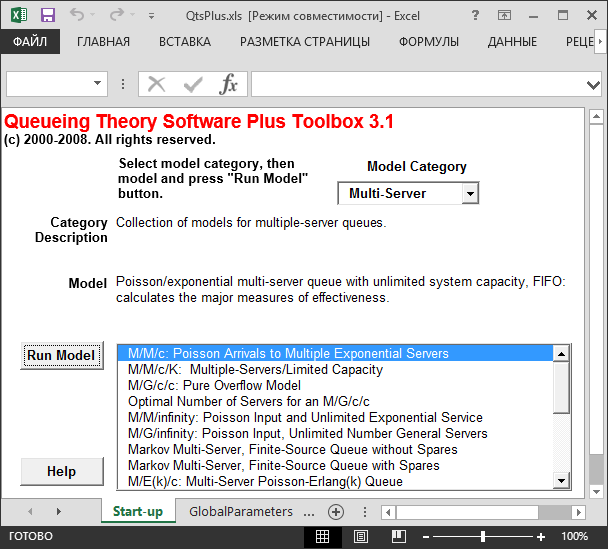
\includegraphics[width = 9\gridunitwidth]{./assets/00-01.png}
        \caption{Головне вікно програми~\textenglish{QtsPlus}}
        \label{fig:setup}
      \end{figure}

      Після запуску моделі відкриється вікно її~налаштувань. У~вікні налаштувань необхідно ввести параметри моделі, надані у~варіанті, а~саме: інтенсивність потоку~$\lambda = \num{2.3}$ та~час~обслуговування~$\mu = \num{2.5}$. Однак, налаштування системи моделювання не~передбачають введення часу обслуговування~$\mu$. Натомість, необхідно ввести значення медіанного часу обслуговування~$1 / \mu$. Щоб~отримати це~значення, його необхідно обчислити зі~значення часу обслуговування~$\mu$:
      \begin{IEEEeqnarray*}{rCl}
        1 / \mu = 1 / \num{2.5} = \num{0.4}.
      \end{IEEEeqnarray*}
      Обчисливши значення, вводимо його разом з~іншими заданими параметрами у~вікно налаштування моделі~(рис.~\ref{fig:setup-model}).

      \begin{figure}[!htbp]
        \centering
        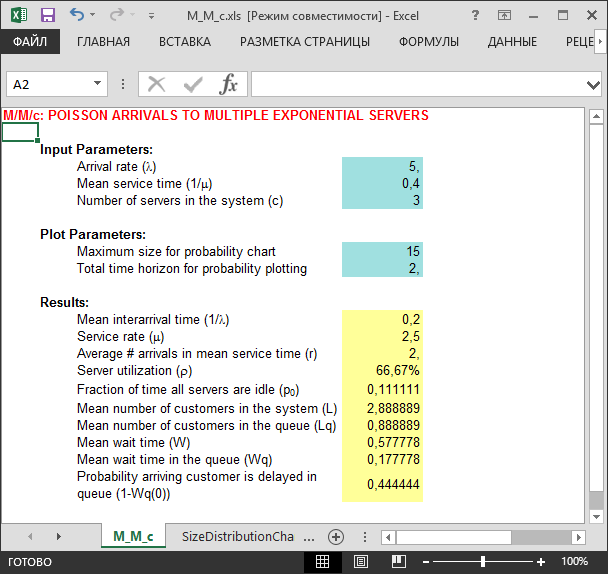
\includegraphics[width = 9\gridunitwidth]{./assets/00-02.png}
        \caption{Головне вікно моделі}
        \label{fig:setup-model}
      \end{figure}

      Ввівши параметри моделі, її~моделювання відбувається автоматично, тому одразу ж~можна переглядати результати. Результати представлені у~вигляді даних та~графіків. Щоб~їх~переглянути, достатньо перейти на~сусідні вкладки, які~містять відповідні дані: діаграму розподілу розміру черги, діаграму розподілу часу очікування в~черзі та~дані для~побудови графіків.

    \subsection{Аналіз графіків розподілів у~системі для~кількості каналів}
      Проаналізуємо графіки розподілу ймовірностей кількості заявок у~системі. Для~цього переходимо у~вкладку~\textenglish{SizeDistributionChart} і~спостерігаємо графік. Далі змінюємо значення кількості каналів у~системі від~1 до~3 і~будуємо графіки для~цих~випадків~(рис.~\ref{fig:size-dist-chart}).

      \begin{figure}[!htbp]
        \begin{subfigure}[b]{6 \gridunitwidth - 0.5 \gridunitwidth}
          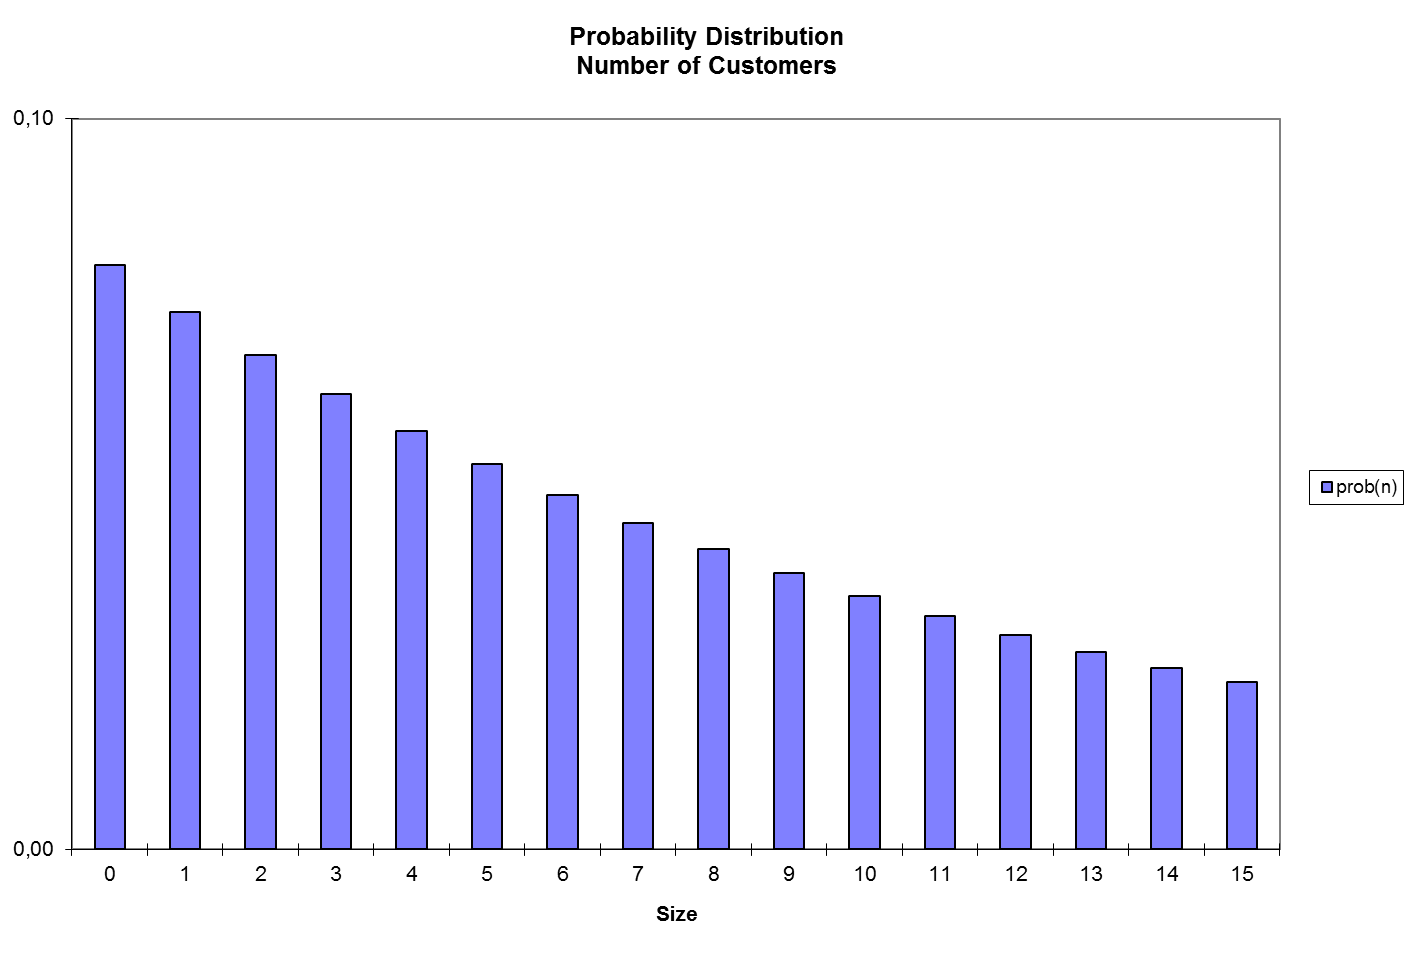
\includegraphics[width = \columnwidth]{./assets/01-01.png}
          \caption{При~1 каналі у~системі}
          \label{subfig:size-dist-chart-01}
        \end{subfigure}%
        \hspace{1 \gridunitwidth}%
        \begin{subfigure}[b]{6 \gridunitwidth - 0.5 \gridunitwidth}
          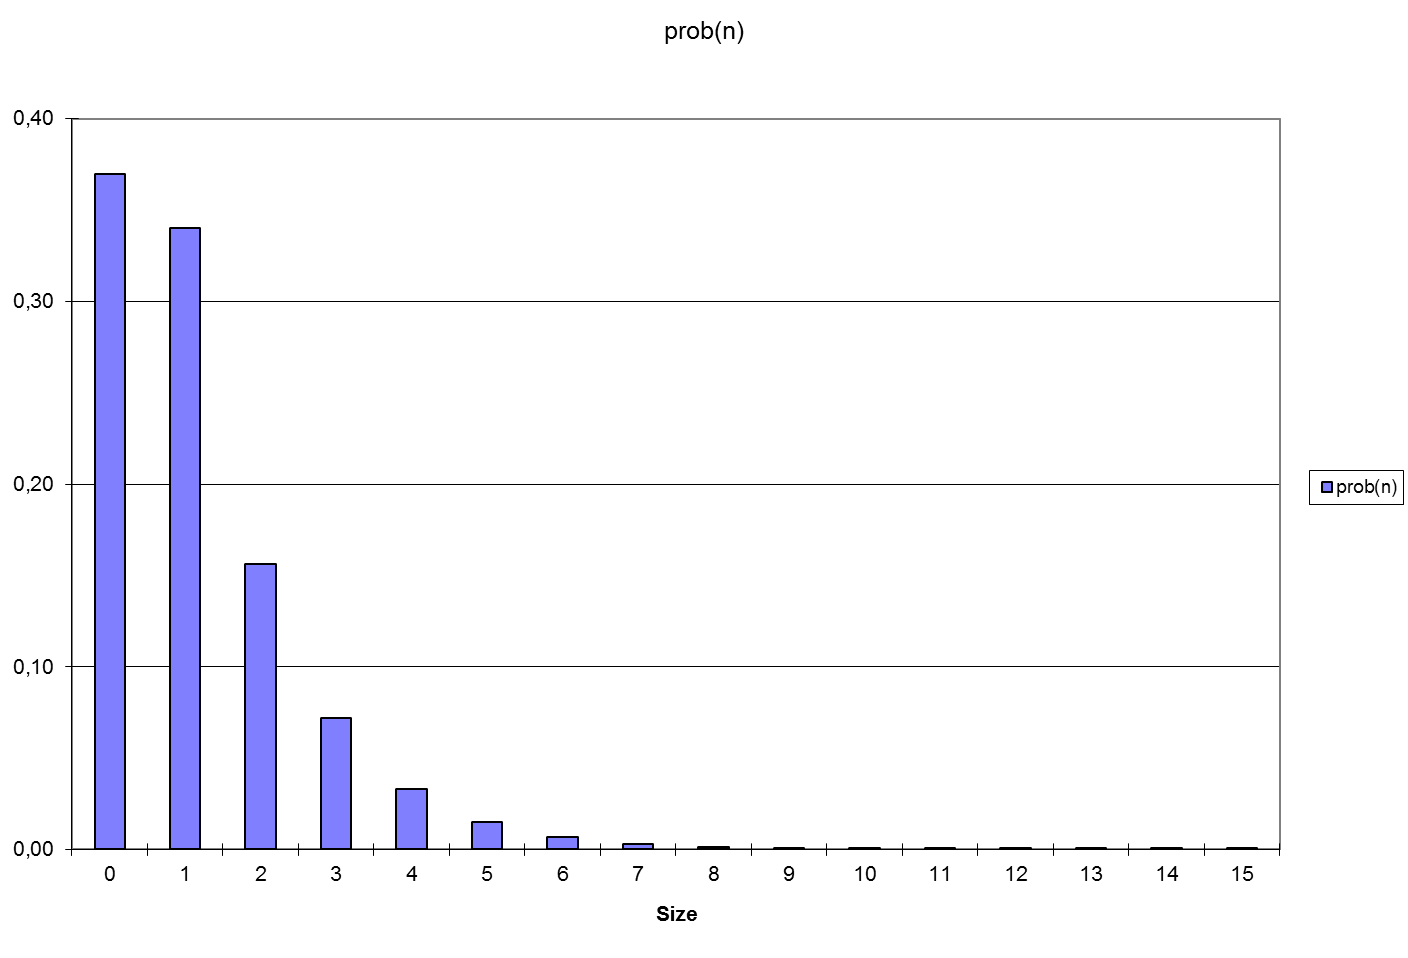
\includegraphics[width = \columnwidth]{./assets/02-01.png}
          \caption{При~2 каналах у~системі}
          \label{subfig:size-dist-chart-02}
        \end{subfigure}
        \begin{subfigure}[b]{6 \gridunitwidth - 0.5 \gridunitwidth}
          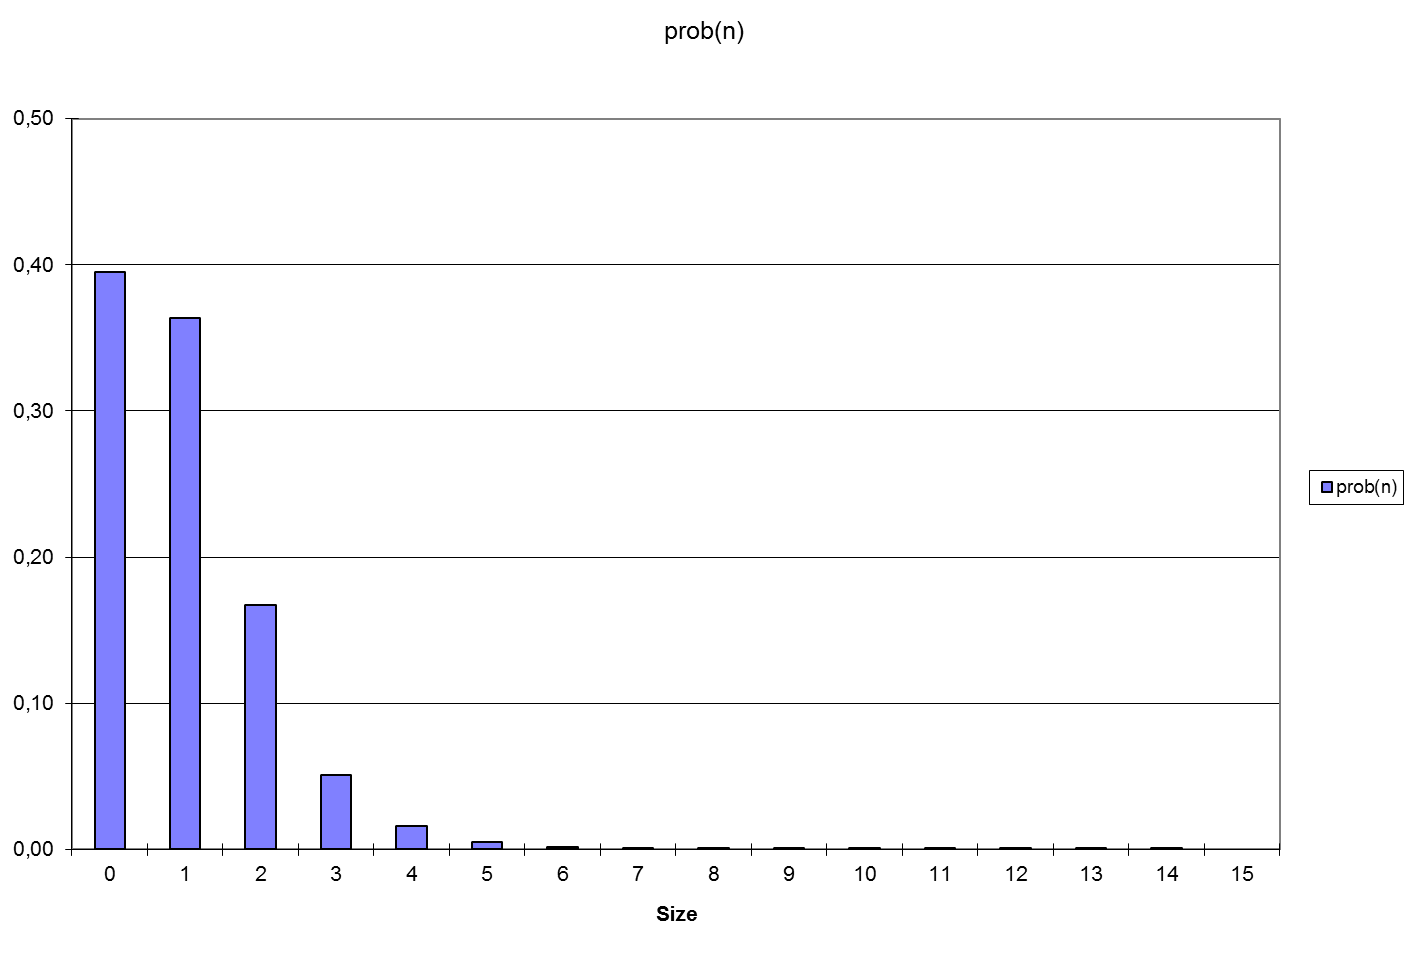
\includegraphics[width = \columnwidth]{./assets/03-01.png}
          \caption{При~3 каналах у~системі}
          \label{subfig:size-dist-chart-03}
        \end{subfigure}
        \caption{Графіки розподілу розмірів черги залежно від~кількості каналів у~системі}
        \label{fig:size-dist-chart}
      \end{figure}

      Як~видно на~графіках, збільшення кількості каналів у~системі суттєво зменшує ймовірність, що~у~черзі буде більше, ніж~2~заявки.

      Тепер проаналізуємо графіки розподілу ймовірностей часу перебування заявок у~системі. Для~цього переходимо у~вкладку~\textenglish{TimeDistributionChart} і~спостерігаємо графік. Далі змінюємо значення кількості каналів у~системі від~1 до~3 і~будуємо графіки для~цих~випадків~(рис.~\ref{fig:time-dist-chart}).

      \begin{figure}[!htbp]
        \begin{subfigure}[b]{6 \gridunitwidth - 0.5 \gridunitwidth}
          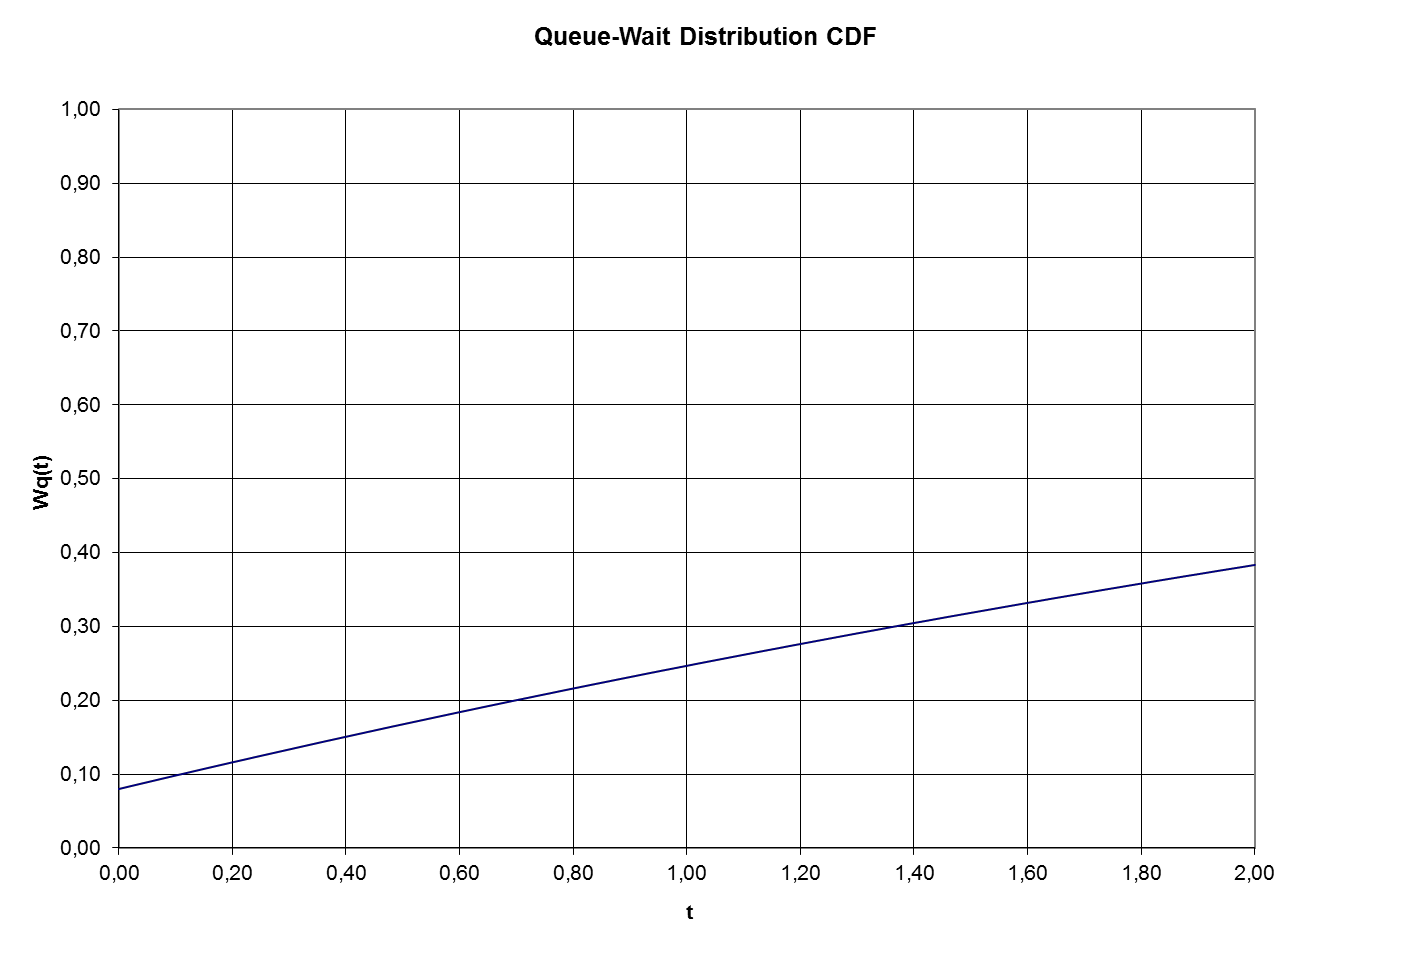
\includegraphics[width = \columnwidth]{./assets/01-02.png}
          \caption{При~1 каналі у~системі}
          \label{subfig:time-dist-chart-01}
        \end{subfigure}%
        \hspace{1 \gridunitwidth}%
        \begin{subfigure}[b]{6 \gridunitwidth - 0.5 \gridunitwidth}
          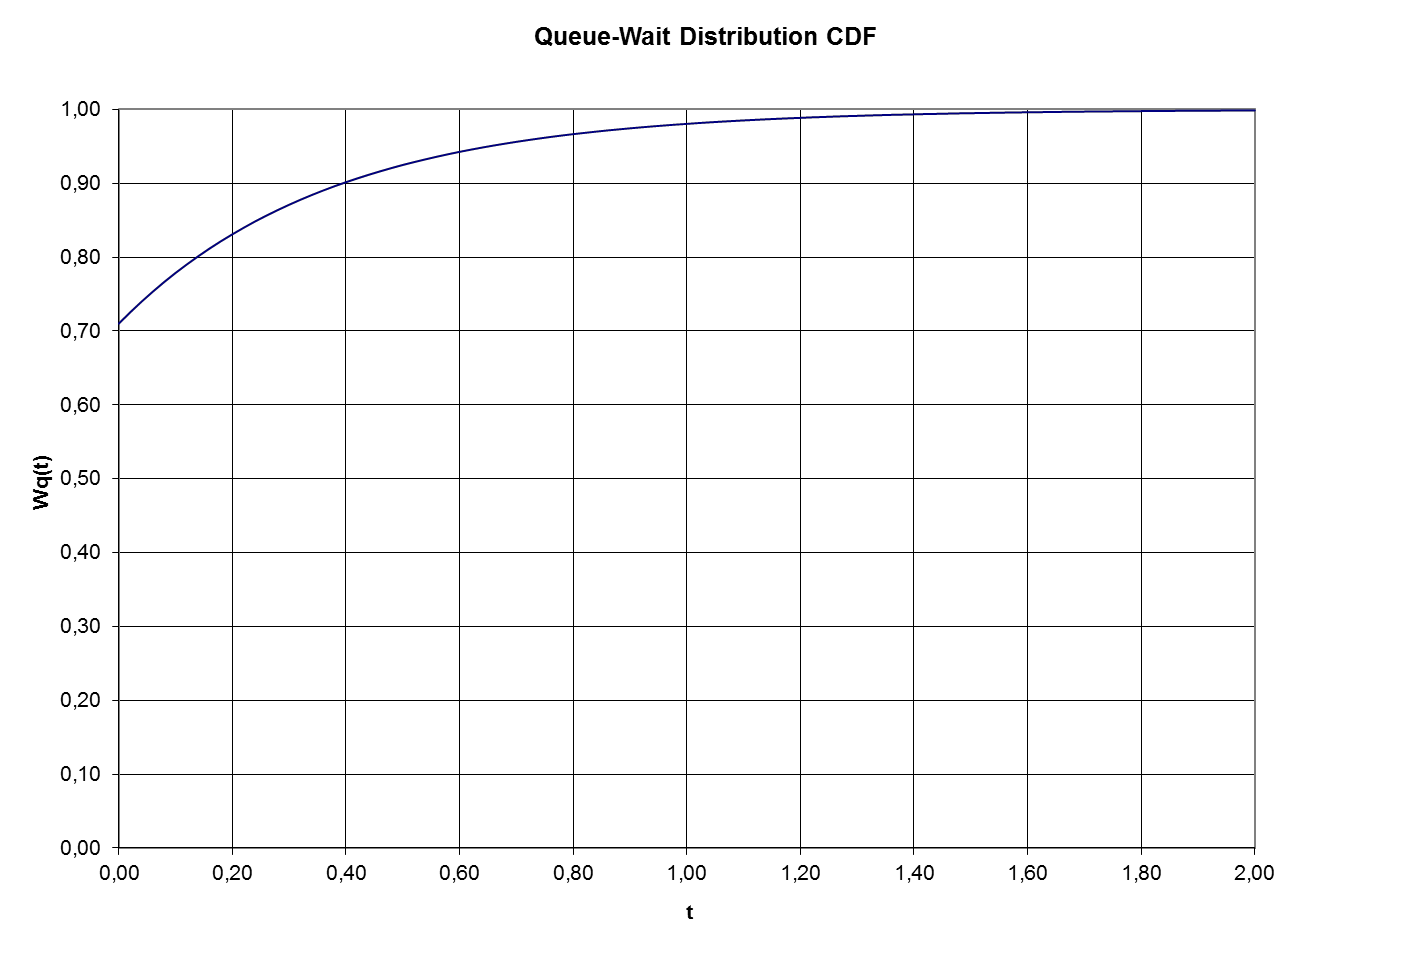
\includegraphics[width = \columnwidth]{./assets/02-02.png}
          \caption{При~2 каналах у~системі}
          \label{subfig:time-dist-chart-02}
        \end{subfigure}
        \begin{subfigure}[b]{6 \gridunitwidth - 0.5 \gridunitwidth}
          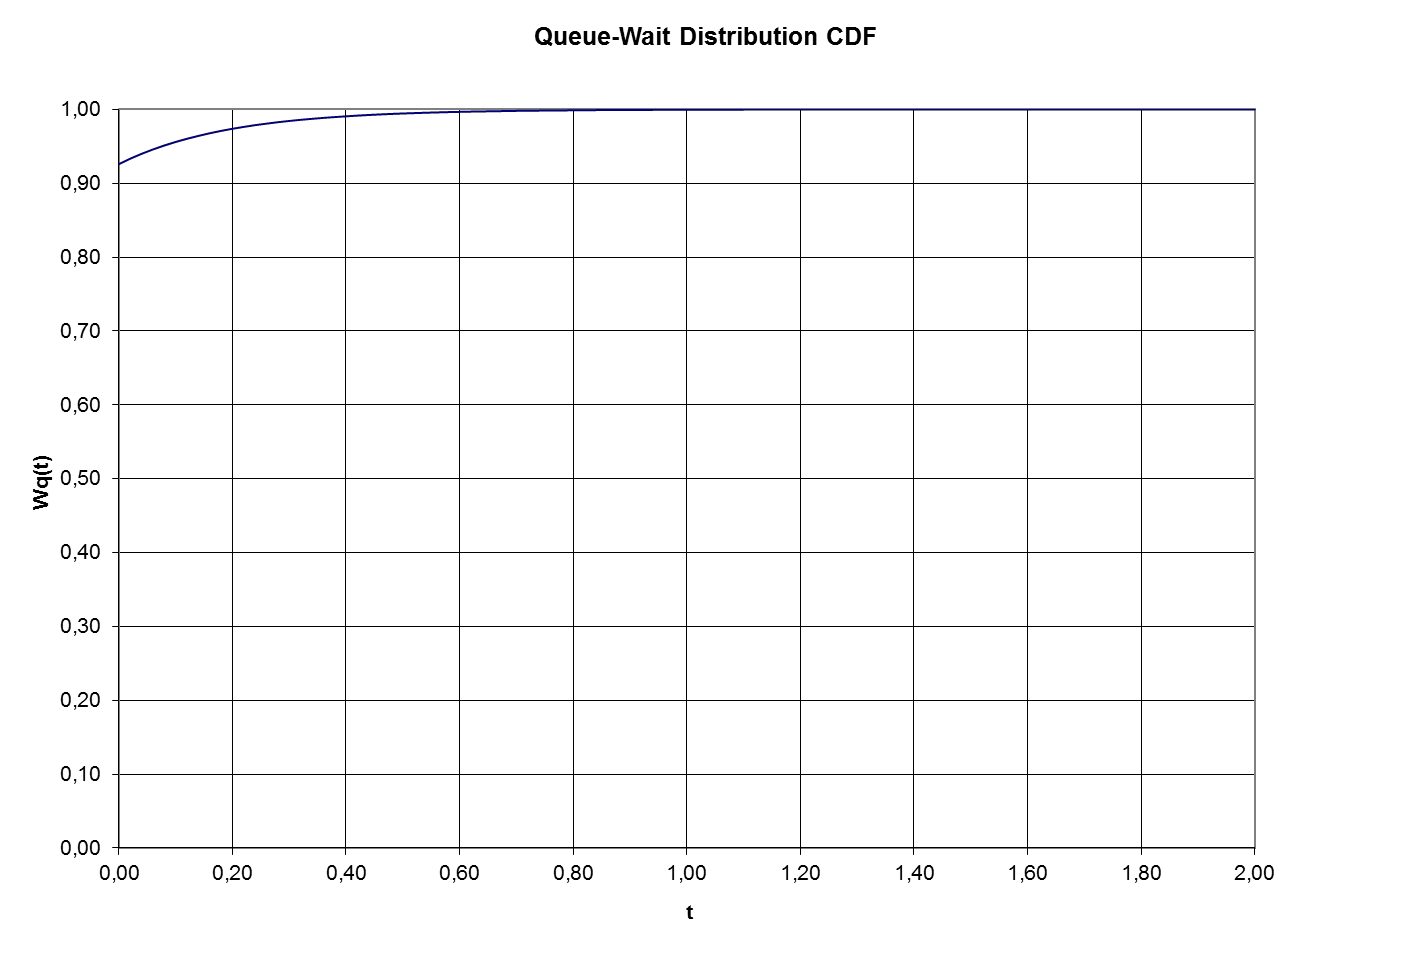
\includegraphics[width = \columnwidth]{./assets/03-02.png}
          \caption{При~3 каналах у~системі}
          \label{subfig:time-dist-chart-03}
        \end{subfigure}
        \caption{Графіки розподілу часу перебування заявок у~системі залежно від~кількості каналів}
        \label{fig:time-dist-chart}
      \end{figure}

      Як~видно на~графіках, збільшення кількості каналів у~системі суттєво збільшує ймовірність (до~90\%), що~заявка проведе в~черзі~0 одиниць часу, тобто миттєво перейде в~обробку.

    \subsection{Аналіз заданого показника залежно від~кількості каналів}
      Завдання варіанту вимагає проаналізувати залежність середнього часу перебування заявок у~системі від~кількості каналів у~системі. Для~цього необхідно провести моделювання для~різних кількостей каналів системи, зібрати значення показника і~занести дані до~відповідної таблиці~(табл.~\ref{tab:wait-in-queue-of-n}).

      \begin{table}[!htbp]
        \centering
        \caption{Залежність середнього часу перебування заявок у~системі від~кількості каналів у~системі}
        \label{tab:wait-in-queue-of-n}
        \sisetup{
          table-format = 1.6,
          table-auto-round = true,
          table-column-width = {8\gridunitwidth - 2\tabcolsep},
          table-number-alignment = right,
          table-text-alignment = right,
        }
        \begin{tabular}{
          v{4\gridunitwidth - 2\tabcolsep}
          S
        }
          \toprule
            {Кількість каналів~$n$} & {Середній час~перебування заявок у~системі~$W_q$} \\
          \midrule
             1 & 4.6 \\
             2 & 0.107357 \\
             3 & 0.014226 \\
             4 & 0.002004 \\
             5 & 0.000263 \\
             6 & 0.000031 \\
             7 & 0.000003 \\
             8 & 0 \\
             9 & 0 \\
            10 & 0 \\
          \bottomrule
        \end{tabular}
      \end{table}

      Зібравши значення середнього часу перебування заявок у~системі залежно від~кількості каналів, візуалізуємо отримані дані~(рис.~\ref{fig:wq-vis}). Видно, що~зі~збільшенням кількості каналів зменшується середній час~перебування заявки у~черзі.

      \begin{figure}[!htbp]
        \centering
        \begin{tikzpicture}
          \datavisualization [
            all axes = {
              grid,
            },
            scientific axes = {
              standard labels,
              width = 11\gridunitwidth,
              height = 14\baselineskip,
            },
            x axis = {
              label = {Кількість каналів~$n$},
            },
            y axis = {
              label = {Середній час~перебування у~черзі~$W_q$},
            },
            visualize as line = dataset1,
            dataset1 = {
              style = {
                mark = x,
              },
            },
            style sheet = vary hue,
          ]
          data [
            set = dataset1,
          ] {
            x, y
             1, 4.6
             2, 0.107357
             3, 0.014226
             4, 0.002004
             5, 0.000263
             6, 0.000031
             7, 0.000003
             8, 0
             9, 0
            10, 0
          };
        \end{tikzpicture}
        \caption{Графік залежності середнього часу перебування заявок у~системі від~кількості каналів у~системі}
        \label{fig:wq-vis}
      \end{figure}

  \section{Висновок}
    Виконуючи дану лабораторну роботу, ми~ознайомились з~пакетом програм розрахунку показників функціонування~\allcaps{СМО} під~назвою~\textenglish{qtsplus-excel} і~засвоїли технології роботи з~цим~пакетом для~визначення показників функціонування~\allcaps{СМО} типу~$M/M/n$.

\end{document}
